In this chapter I will present the two phases learning process utilized by the fully connected neural network (FCNet) to maximize the agents utility. Afterwards there will be a brief description of the 5 environments I am going to study (one per taxation analyzed) and my conjecture on how the agents will respond to these taxation.


\section{Experiment Setup}

After understanding the Foundation framework and the process used by RL to optimize a policy we can focus on the model used. In the paper used as a reference the authors used a combination of a convolutional neural network and a LSTM \cite{zheng2020ai}. This could grant them good spatial information from the CNN and a memory buffer from the LSTM. These feature are sensate because there is the need of process a map and because the agents share the same network.

In the experiments, however, it was used a fully connected neural network that do not share the same feature as the one above. The complete stucture of the model is shown in Table \ref{tab:Fcnet}. 


\begin{table}[h!]
    \begin{tabular}{llll}
	Model: "FCNet"            &                    &          &                            \\ \hline
	Layer (type)              & Output Shape       & Param \# & Connected to               \\ \hline
	observations (InputLayer) & {[}(None, 1260){]} & 0        &                            \\ \hline
	encoder (Encoder)         & (None, 256)        & 389632   & observations{[}0{]}{[}0{]} \\ \hline
	fc\_out (Dense)           & (None, 50)         & 12850    & encoder{[}0{]}{[}0{]}      \\ \hline
	value\_out (Dense)        & (None, 1)          & 257      & encoder{[}0{]}{[}0{]}      \\ \hline
	Total params: 402,739     &                    &          &                            \\
	Trainable params: 402,739 &                    &          &                            \\
	Non-trainable params: 0   &                    &          &                            \\ \hline
    \end{tabular}
    \caption{\label{tab:Fcnet} Fully connected neural network utilized.}
\end{table}


This setup might encur in a loss of efficiency for plenty of reasons. First of all, as said before, the feature of the LSTM/CNN are missing. Then due to lack of resources it was not possible to do a proper hyper parameter tuning, probably leading to inefficiencies. However, as we will see, the FCNet can provide us with meaningful results, in particular the agents will show emerging behaviors and specialization. These are feature that were also finded in the paper by Zhang and Trott, the difference is present in the efficiency of the agents that is lower for the model used here.

There are many parameters that have to be set at this stage (for a semi-complete list check the appendix \textcolor{red}{appendice}). A first part of these values are related to the training, while a second part to the environment. I would like to stress some of the latter parameters, to better undersand the simulation.

First the skill levels, these are set to be different for each agent, the skill is the amount of coins received when building an house. The set of 4 skills is fixed and these are taken from a pareto distribution. Namely the values are (11.3; 13.3; 16.5; 22.2). These value are always assinged to the same starting location in the map, thus the agent starting in the bottom right will always have the highest skill and so on. Other important parameters are the episode lenght \( H \) which is set to 1000 time steps, the resource respawn probability which is set to 1\% per timestep and the inital coin endowment that is set to 0.

Once defined the environment is defined it is possible to start the training, this will happen in two phases. The first phase to introduce labour, and the second to introduce the taxation.

\section{Phase 1 training}

The first training phase is necessary in order to get the FCNet \ref{tab:Fcnet} accustomed to the world dynamics and avoid falling into unoptimal behavior once disincentives factors are introduced. These two factors, as already discussed, are labour costs and taxation. In this first phase the interest is in getting the agent accustomed to the labour costs, while the taxes are completely removed and will be investigated in the second phase of training. 


\begin{figure}[h!]
    \centering
    \linespread{.9} 
    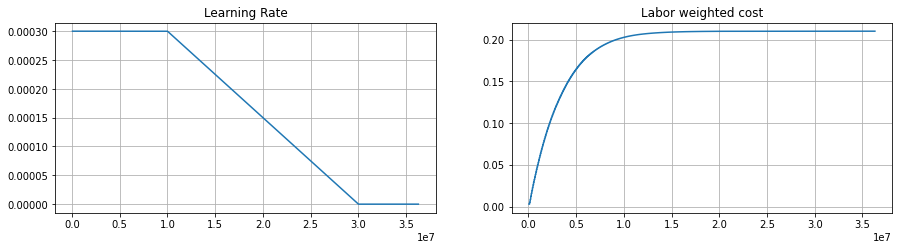
\includegraphics[width=0.95\textwidth]{Resources/imgs/LR_phase1.png}
    \caption[Learning rate and Labor weighed cost for Phase 1 training: ]%
    {\label{img:lr_phase0}Learning rate and Labor weighed cost for Phase 1 training: \small \textit{this was the schedule for respectively the learning rate and the labor cost in the phase 1 of the training, here the learning rate goes to 0 because we don't seek convergence now.}}
\end{figure}

The training agenda is built to run for a total of 30M time-steps, as we can see from Figure \ref{img:lr_phase0} the learning rate is set to be at 1e-4 for 10M steps then it linearly reduces to 0 in 20M time-steps. While the labour weight increases following the function:

\begin{equation}
    \vartheta_k = 1- exp\left(- \frac{\textit{episode completitions}}{\textit{energy warm-up constant (k)}}\right)
\end{equation}

where the warm-up constant is set to 10000. This setup gives the FCNet time to learn how to respond properly to the dis-utility generated by the labor. 



\begin{figure}[h!]
    \centering
    \linespread{.9} 
    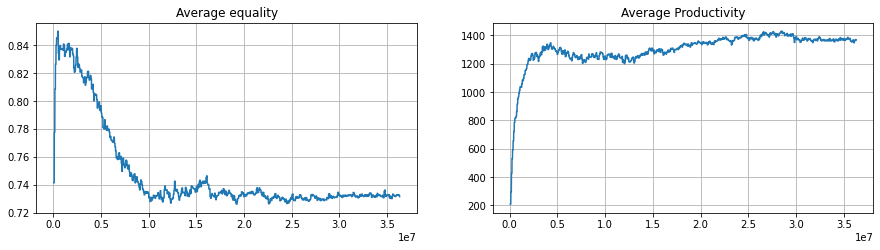
\includegraphics[width=0.95\textwidth]{Resources/imgs/FCNET_prod_phase1.png}
    \caption[Equality and Productivity during Phase 1:  ]%
    {\label{img:prod_phase0}Equality and Productivity during Phase 1: \small \textit{here we have the evolution of equality between agents and total production in the training of phase 1}}
\end{figure}


In Figure \ref{img:prod_phase0} we can see two of the most important variables that we are considering. On the left we have the average equality, this value is calculated by the following formula:

\begin{equation}
    equality(\mathbf{x^c_{t}}) = 1 - \frac{N}{N-1} \frac{\sum^N_{i=1}\sum^N_{j=1}| x^c_{i,t} - x^c_{j,t}|}{2N\sum^N_{i=1}x^c_{i,t}}
\end{equation}

with \( 0 < equality(\mathbf{x^c_{t}}) < 1 \), this function returns 1 if the endowments are equally split between the N (4) agents, and 0 if only one agent owns all of the coin in the economy. What we see is that after 36M time-steps the equality settled around 0.73, this is justified by the difference in coin endowment between the agent with the highest skill (Agent 0 in Figure \ref{img:p0_brakedown}) and the other agents. And we see that the average productivity of he economy settles around 1400. 


\begin{figure}[h!]
    \centering
    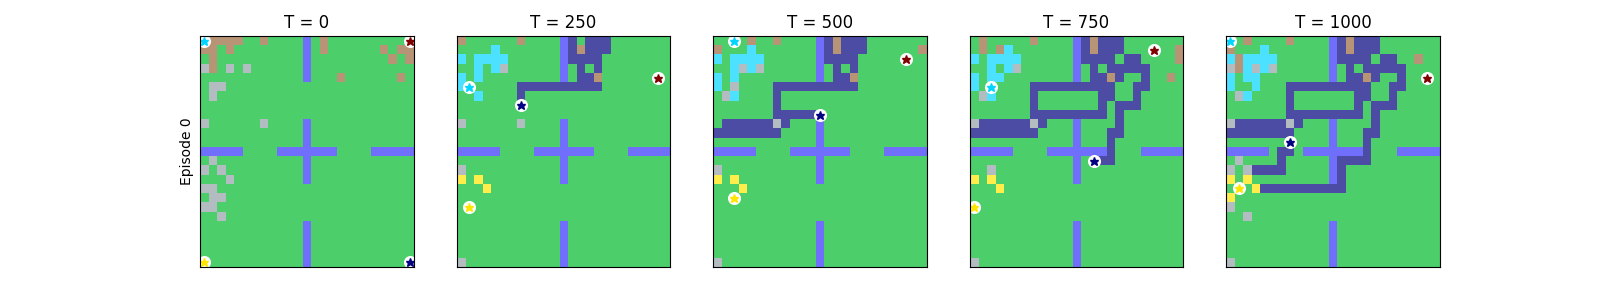
\includegraphics[width=0.95\textwidth]{Resources/imgs/Figure_1.png}
    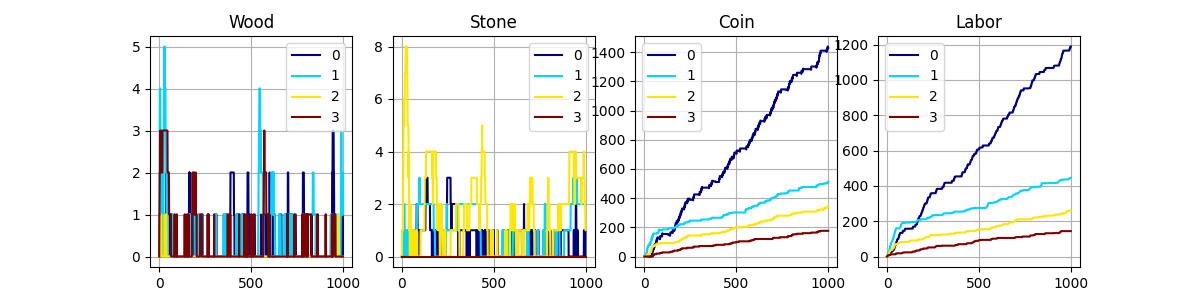
\includegraphics[width=0.80\textwidth]{Resources/imgs/Figure_2.png}
    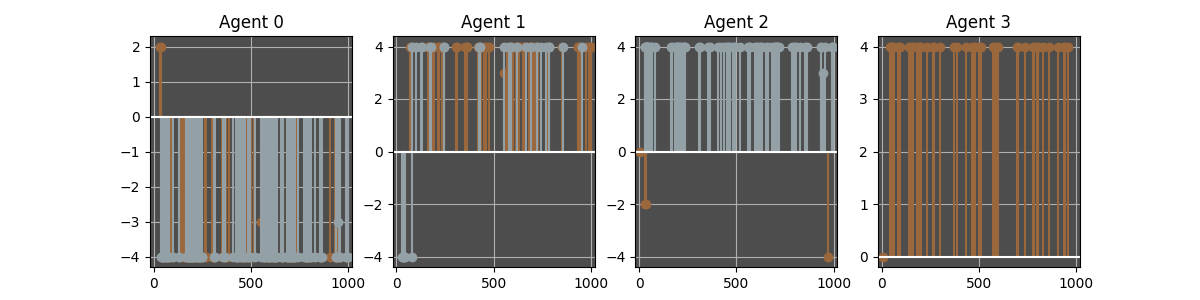
\includegraphics[width=0.80\textwidth]{Resources/imgs/Figure_3.png}
    \caption[Phase 1 full brake down: ]%
    {\label{img:p0_brakedown}Phase 1 full brake down: \small \textit{this is a more complete overview of one random simulation crated using the weights at the end of phase 1 training}}
\end{figure}


The results obtained so far are not important for the final analysis since there were no criterion used to stop the training other than a time constraint. This means that the FCNet might have not reached convergence and an optimal policy. However we can keep these results in mind as a benchmark for the phase 2 trainig as we will use the parameters obtained to carry on the training.


\section{Phase 2 Trainig}

    
In the second phase of the training the learning rate schedule is changed to be 3e-4 for the first 35M time-steps and then will linearly decrease to 1e-6 in a span of 15M time-steps. This will grant a faster learning rate in the inital part of the trainig when the FCNet will suffer a huge decrease in efficiency due to the introduction of the taxation. 

The starting point for this second phase are the weights obtained from phase 1, and the training will be formed of five different simulations diverging from this inital state. These simulation are: US taxation, Italian Taxation, free market, Communism and Flat Tax.

\subsection{Free Trade}

Free trade is the first and simplest kind of simulation that we can carry on starting from the result in phase 1. This training consist in keep training the FCNet without imposing any kind of taxation. 

It is reasonable to belive that the result of this first training should produce a more productive economy since the agent's utility function is positive in marginal coin endowment. However the equality between agents might suffer from a higher production.

\subsection{US taxation}

The second kind of taxation that will is used is the US taxation. This is based on the 2018 Federal brachets and percentages. In particular we can see from Table \ref{tab:us_tax} the detailed stucture. 

\begin{table}[h!]
\begin{adjustbox}{max width=\textwidth}
    \begin{tabular}{llllllll}
        \hline
    Bracket in \$   & 0-9700 & 9700-39475 & 39475-84200 & 84200-160725 & 160725-204100 & 204100-510300 & 510300+ \\
    Bracket in Coin & 0-9.7  & 9.7-39.5   & 39.5-84.2   & 84.2-160.7   & 160.7-204.1   & 204.1-510.3   & 510.3+  \\
    Tax*            & 10\%   & 12\%       & 22\%        & 24\%         & 32\%          & 35\%          & 37\%\\
    \hline
    \end{tabular}
\end{adjustbox}
    \caption[2018 US federal tax system:]%
    {\label{tab:us_tax}2018 US federal tax system: \small \textit{this is the proportional system that was in place in the US in 2018, notice that the tax is marginal (i.e. if you are in the second bracket you will pay 970\$ + 12\% of the amount above 9700\$) }}
\end{table}

With the introduction of these lump sum tax plus redistribution is easy to conclude that there might me an increase in equality, however this migh produce a negative effect on total production since the high-skilled agent are disincentivised to produce.

\subsection{Italian Taxation}

As of the US's the Italian is a marginal system with brackets, however in this case the fiscal pressure is higer and the brachets smaller. As a reference it was used the 2020 INPS brachets and percentages (Table \ref{tab:ita_tax}). However, the brackets were calculated as if in dollars, so all the values were multiplied by 1.1575, the exchange rate at October 1st 2021.


\begin{table}[h!]
    \begin{adjustbox}{max width=\textwidth}
        \begin{tabular}{llllll}
            \hline
        Bracket in \EURcr   & 0-15000 & 15000-28000 & 28000-55000 & 55000-75000 & 75000+ \\
        Bracket in Coin & 0-17  & 17-32  & 32-63  & 63-86   &  86+   \\
        Tax*            & 23\%   & 27\%       & 38\%        & 41\%         & 43\%       \\
        \hline
        \end{tabular}
    \end{adjustbox}
        \caption[2018 US federal tax system:]%
        {\label{tab:ita_tax}2020 INPS tax system: \small \textit{this is the proportional system that was in place in the Italy in 2020, notice that the tax is marginal (i.e. if you are in the second bracket you will pay 3450\EURcr + 27\% of the amount above 15000\EURcr) }}
    \end{table}



In this case there is an even higher pressure, wich might push toward higher equality and lower total production.


\subsection{Communism}

Communism is the opposite to Free market, in this simulation the fiscal pressure is 1, meaning that every 100 timestep all the agents are taxed for the entire amount of coins they own and then redistibuted. This system will probably deliver the loewst production and the highest equality.

\subsection{Flat tax}



\section{Training Results}


\begin{figure}[h!]
    \centering
    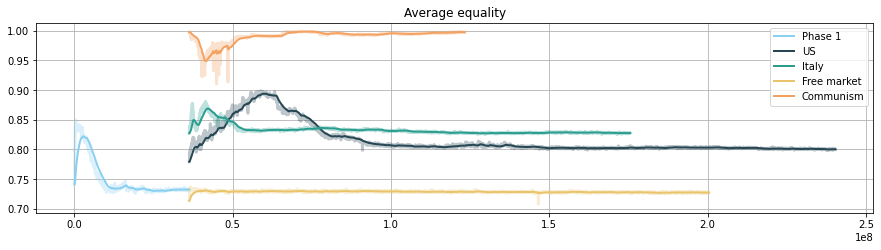
\includegraphics[width=0.95\textwidth]{Resources/imgs/equality_training.png}
    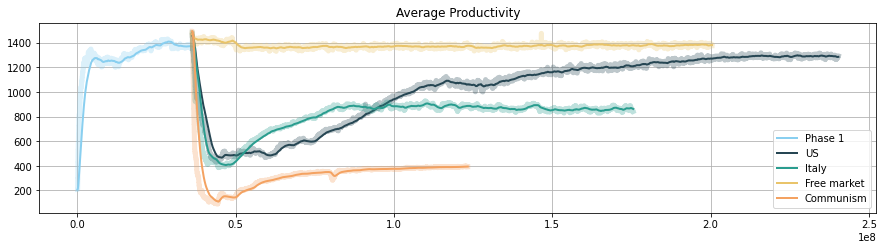
\includegraphics[width=0.95\textwidth]{Resources/imgs/productivity_training.png}
    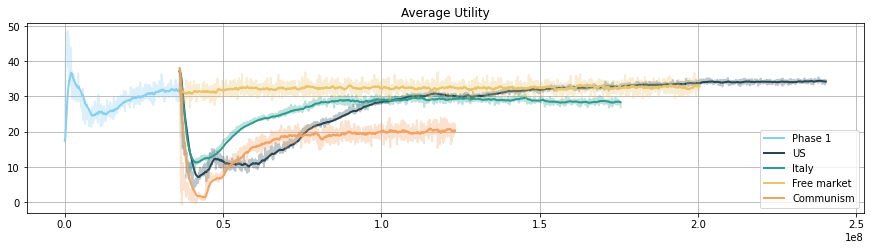
\includegraphics[width=0.95\textwidth]{Resources/imgs/utility_training.png}
    \caption[Phase 1 full brake down: ]%
    {\label{img:p1_brakedown}Phase 2 full brake down: \small \textit{this is a more complete overview of one random simulation crated using the weights at the end of phase 1 training}}
\end{figure}
